\chapter{Generelle statistiske begreber}
I dette appendiks introduces nogle definitioner og sætninger, som anvendes igennem rapporten.
%
\begin{thm}[Slutsky's Theorem] \label{thm:slutsky}
Hvis $X_n \overset{d}{\rightarrow} X$ og $Y_n \overset{p}{\rightarrow} c$, hvor $X$ er en stokastisk variabel og $c$ er en konstant, da gælder, at
\begin{align*}
& X_n + Y_n \overset{d}{\rightarrow} X+c \\
& X_n Y_n \overset{d}{\rightarrow} cX \\
& \frac{X_n}{Y_n} \overset{d}{\rightarrow} \frac{X}{c}, \quad \text{forudsat at } P(c=0)=0.
\end{align*}
\end{thm}
Sætning \ref{thm:slutsky} tillader at finde grænsefordelingen af $X_n$ og sandsynlighedsgrænsen af $Y_n$ separat.
%
\begin{defn}[Konveks mængde] \label{defn:konveksm}
En mængde \(\mathcal{C} \subseteq \R^p\) er konveks, hvis der for alle \(\tbeta, \tbeta' \in \mathcal{C}\) og alle skalarer \(s \in \sbr{0,1}\) gælder, at alle vektorer på formen
\begin{align*}
\tbeta \del{s} = s \tbeta + \del{1-s} \tbeta'.
\end{align*}
tilhører \(\mathcal{C}\).
\end{defn}
%
\begin{defn}[Konveks funktion] \label{defn:konveksfkt}
En funktion \(f: \ \R^p \rightarrow \R\) er konveks, hvis der for \(\tbeta\), \(\tbeta'\) i definitionsmængden af \(f\) og enhver skalar \(s \in \del{0,1}\) gælder
\begin{align*}
f \del{\tbeta \del{s}} = f \del{s \tbeta + \del{1-s} \tbeta'} \leq s f\del{\tbeta} + \del{1-s} f\del{\tbeta'}.
\end{align*}
\end{defn}
Geometrisk medfører uligheden at akkorden mellem \(f \del{\tbeta}\) og  \(f \del{\tbeta'}\) ligger over grafen af \(f\), som illustreres på figur \ref{fig:konveks}.
Uligheden sikrer, at en konveks funktion ikke kan have et lokalt minimum, som ikke også er et globalt minimum.
%
\begin{figure}[H]
\centering
\scalebox{1.2}{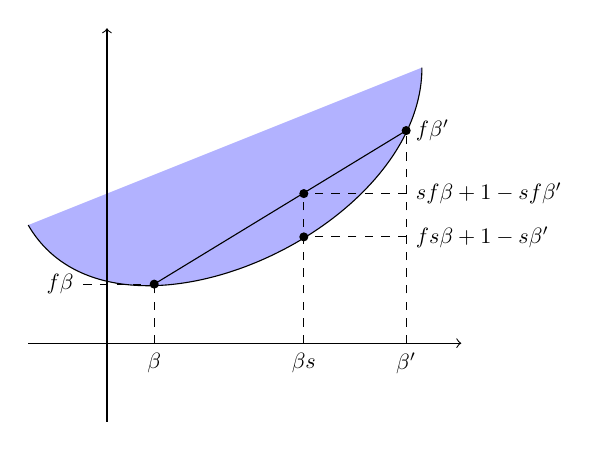
\begin{tikzpicture}
\draw (-1,1.5) to[out=300,in=270] (4,3.5)[fill= blue!30];
\draw [->] (-1,0) -- (4.5,0); % x-aksen
\draw[->] (0,-1) -- (0,4); % y-aksen
\draw (0.6,0.75) -- (3.80,2.7);
\draw [fill] (0.6,0.75) circle [radius=0.05];
\draw [fill] (3.80,2.7) circle [radius=0.05];
\draw [fill] (2.5,1.9) circle [radius=0.05];
\draw [fill] (2.5,1.35) circle [radius=0.05];
\draw [dashed] (-0.3,0.75) node [left] {\scalebox{0.8}{$f \del{\beta}$}} -- (0.6,0.75);
\draw [dashed] (0.6,0) node [below] {\scalebox{0.8}{$\beta$}} -- (0.6,0.75);
\draw [dashed] (2.5,0) node [below] {\scalebox{0.8}{$\beta \del{s}$}} -- (2.5,1.9);
\draw [dashed] (3.80,0) node [below] {\scalebox{0.8}{$\beta'$}} -- (3.80,2.7);

\draw [dashed] (3.80,2.7) node [right] {\scalebox{0.8}{$f \del{\beta'}$}} -- (3.80,2.7);
\draw [dashed] (3.80,1.9) node [right] {\scalebox{0.8}{$ sf \del{\beta} + \del{1-s} f \del{\beta'}$}} -- (2.5,1.9);
\draw [dashed] (3.80,1.35) node [right] {\scalebox{0.8}{$f \del{s \beta + \del{1-s} \beta'}$}} -- (2.5,1.35);
\end{tikzpicture}
}
\caption{For en konveks funktion ligger linjen \(s f \del{\beta} + \del{1-s} f \del{\beta'}\) altid over funktionsværdien \(f \del{s \beta + \del{1-s} \beta'}\).} \label{fig:konveks}
\end{figure}
%
\begin{defn}[General position] \label{defn:general_position}
Søjlerne i en \(n \times p\) matrix \(\X\) siges at være i general position, hvis der ikke findes et  \(k\)-dimensionel underrum \(L \subset \R^n\), hvor \(k < \min \cbr{n,p}\), som indeholder mere end \(k+1\) elementer af mængden \(\cbr{\pm \x_1, \ldots, \pm \x_p}\) med undtagelse af par af antipodal punkter.
Sagt med andre ord: det affine spænd af \(k+1\) punkter \(s_1 \x_{i_1}, \ldots, s_{k+1} \x_{i_{k+1}}\) indeholder ikke ethvert element af mængden \(\cbr{\pm \x_i : \ i \neq i_1, \ldots, i_{k+1}}\) for ethvert fortegn \(s_1, \ldots, s_{k+1} \in \cbr{-1,1}\).
\end{defn}
%
Antagelsen om at søjlerne i \(\X\) er i general position er svag.
Langt svagere end antagelsen om at \(\text{rang} \del{\X} = p\).
Hvis indgangene af \(\X\) er fra en kontinuert sandsynlighedsfordeling på \(\R^{np}\), da er søjlerne i \(\X\) i general position næsten sikkert uanset størrelsen af \(n\) og \(p\) \citep{lasso_unique}. 
At søjler i \(\X\) er i generel position, sikrer at lasso løsningen er entydig \citep{lasso_unique}.
%
\begin{defn}[Rod-n-konsistent estimator] \label{def:rodn}
Estimator \(\widehat{\tbeta}\) er rod-n-konsistent hvis
\begin{align*}
\widehat{\tbeta}  - \tbeta^* = O \left( \frac{1}{\sqrt{n}} \right).
\end{align*}
\end{defn}
\newpage
\begin{defn} \label{defn:supp}
Antag \(f: \X \rightarrow \R\), hvor \(\X\) er en arbitrær mængde.
Støtten af \(f\), som skrives \(\text{supp} \del{f}\), er en mængde af punkter i \(\X\), hvor \(f\) er ikke-nul
\begin{align*}
\text{supp} \del{f} = \cbr{x \in \X \given f \del{x} \neq 0}.
\end{align*}
\end{defn}
%
%
\begin{defn}[En autoregressiv model af orden $p$] \label{def:ar}
En autoregressiv model af orden $p$, som betegnes AR($p$), er givet ved
\begin{align*}
y_t = \phi_1 y_{t-1} + \phi_2 y_{t-2} + \dots + \phi_p y_{t-p} + \omega_t, \qquad t = p+1, \dots, T,  
\end{align*}
hvor $y_t$ er stationær og $\phi_1 , \phi_2, \dots, \phi_p $ er konstanter  $\del{ \phi_p \neq 0}$ og $\omega_t \sim \text{iid}\del{0, \sigma_\omega^2}$.  
\end{defn}
%
\begin{defn}[Jarque-Bera test] \label{def:jbtest}
Betragt \(\hyp_0: \) data er normalfordelt imod \(\hyp_1:\) data er ikke normalfordelt.
Teststørrelsen for Jarque-Bera testen er givet ved
\begin{align*}
\text{JB} = \frac{n-p+1}{6} \del{S^2 + \frac{1}{4} \del{C-3}^2},
\end{align*}
hvor \(n\) er antallet af observationer, \(S\) er den empiriske skewness, \(C\) er den empiriske kurtosis og \(p\) er antallet af prædiktorer.
\end{defn}
Under \(\hyp_0\) følger teststørrelsen \(\text{JB}\) en \(\chi_{\del{2}}^2\)-fordeling.
For et signifikant niveau \(\alpha\), afvises hypotesen hvis \(\text{JB} > \chi_{1-\alpha,2}^2\), hvor \(\chi_{1-\alpha,2}^2\) er en \(1 - \alpha\) kvantil af \(\chi^2\)-fordelingen med \(2\) frihedsgrader.
%
\begin{defn}[Ljung-Box test] \label{def:lbtest}
Betragt \(\hyp_0 :\) de første \(h\) autokorrelationer er nul imod \(\hyp_1 :\) de første \(h\) autokorrelationer er forskellig fra nul.
Teststørrelse for Ljung-Box testen er givet ved
\begin{align*}
\text{LB} = n \del{n +2} \sum_{k=1}^h \frac{\widehat{\rho}_k^2}{n-k},
\end{align*}
hvor \(n\) er antallet af observationer, \(\widehat{\rho}_k^2\) er den empiriske autokorrelation i lag \(k\) og \(h\) er antallet af lags som testes.
\end{defn}
Under \(\hyp_0\) følger teststørrelsen \(\text{LB}\) en \(\chi_{\del{h}}^2\)-fordeling.
For et signifikant niveau \(\alpha\), afvises hypotesen hvis \(\text{LB} > \chi_{1-\alpha,h}^2\), hvor \(\chi_{1-\alpha,h}^2\) er en \(1 - \alpha\) kvantil af \(\chi^2\)-fordelingen med \(h\) frihedsgrader.